本システムは大きく分けて3つの機能によって成り立っている.
それは,グラフデータ管理機能,グラフデータ入力補助機能,グラフデータ可視化機能の3つの機能である.
それぞれの機能について\ref{subsec:kanri}節,\ref{subsec:hojo}節,\ref{subsec:kasi}節で説明する.

\subsection{グラフデータ管理機能}\label{subsec:kanri}
グラフデータ管理機能は,学習者と指導者のグラフデータを管理する機能で,クライアントのフォームから入力されたコンセプトマップの親子に関するデータをAPIを用いてグラフデータへと変換しグラフデータベースへとデータを登録する.
また,クライアントからグラフデータを要求された場合,グラフデータをAPIを用いてJSON形式で返答する.

グラフデータ管理機能が使用するAPIは以下のとおりである.

\begin{itemize}
    \item /create/json \\
    - 与えられたJSON形式のデータをグラフデータベースで利用できるJSON形式のデータに変換し,データを登録しその結果をJSON形式で返答する.

    \item /get/all\_graphs \\
    - グラフデータベースに登録されているすべてのグラフデータをJOSN形式で返答する.

    \item /create/score \\
    - 指定されたユーザと教科の点数登録を行う.

    \item /get/score \\
    - 指定された教科に紐づくすべての点数を返答する.

    \item /get/score/\<username\> \\
    - 指定されたユーザに関する教科の得点を返答する.

    \item /get/subject/\<subject\> \\
    - 指定されたユーザが受験した科目と点数を返答する.

    \item /delete/\<string:node\_name\> \\
    - 指定されたノードを削除する.

    \item /delete/all \\
    - すべてのノードを削除する.
    
\end{itemize}

これらのAPIを利用することにより本システムはグラフデータベースとコンセプトマップを紐づけて利用している.
\newpage

\subsection{グラフデータ入力補助機能}\label{subsec:hojo}
グラフデータ入力補助機能は,クライアントでJSON形式のグラフデータを入力補助する機能である.
この機能は指導者が用いる機能で,新規にグラフデータを入力する場合に用いる.
グラフデータは,最低でも属性,親ノード,子ノードの一セットを入力する必要がある.
そのためテキストベースの従来のデータ入力フォームでは,関係性など誤って入力する可能性がある.
そこで本機能では入力フォームを階層構造で入力可能なUIとして提供し,入力誤りを減らすようにしている.
また,本入力フォームはドラック&ドロップや編集メニューを用い,入力データを階層表示し操作できる.
これにより,指導者は関係性を整理しながらグラフデータを入力することが可能である.

グラフデータ入力補助機能のGUIを図\ref{fig:hojo}に示す.

\begin{figure}[htbp]
\begin{center}
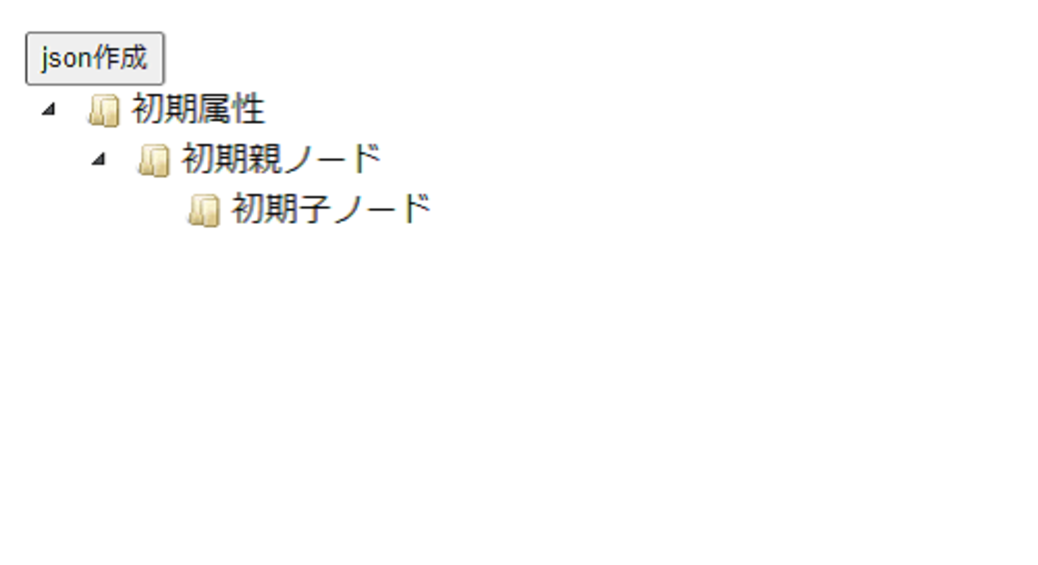
\includegraphics[width=10cm]{img/hojo.eps}
\end{center}
\caption{グラフデータ入力補助機能初期状態}
\label{fig:hojo}
\end{figure}

図\ref{fig:hojo}は初期状態で,図のような木構造な入力フォームを提示する.
初期属性とは第\ref{chap:conceptmap}章の図\ref{fig:example_concept}で示した植物に該当する.
初期親ノードは被子植物,初期子ノードはサクラに該当する.
\newpage
各々の階層は図\ref{fig:hojo_change_name}のようにして各ノードを右クリックすることによりメニューが表示される.

\begin{figure}[htbp]
\begin{center}
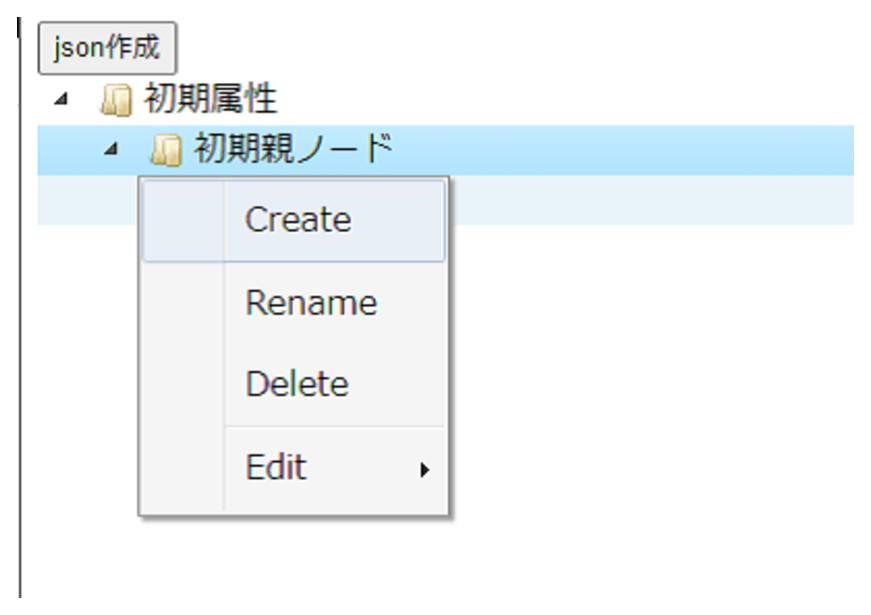
\includegraphics[width=10cm]{img/hojo_change_name.eps}
\end{center}
\caption{グラフデータ入力補助機能編集状態}
\label{fig:hojo_change_name}
\end{figure}

\newpage
メニューはCreate, Rename, Delete, Editの四種類あり,それぞれノードの新規作成,ノードの名前変更,ノードの削除,ノードの編集を意味する.
Editについては,図\ref{fig:hojo_edit}のようにして,Cut, Copy, Pasteが存在し,それぞれノードの切り取り,ノードのコピー,ノードの貼り付けが可能である.

\begin{figure}[htbp]
\begin{center}
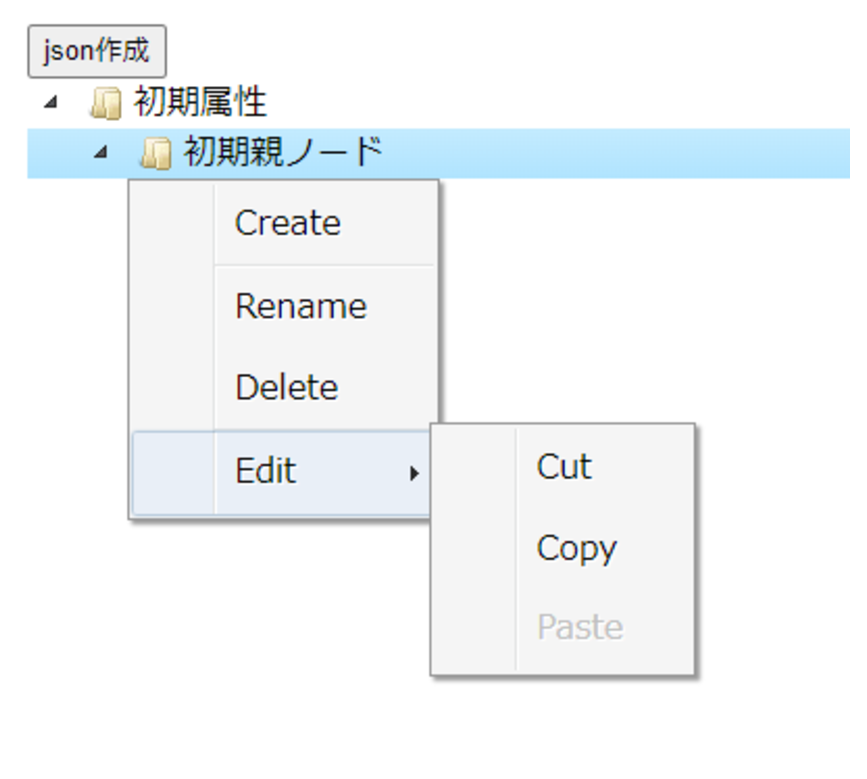
\includegraphics[width=9cm]{img/hojo_edit.eps}
\end{center}
\caption{グラフデータ入力補助機能 Editについて}
\label{fig:hojo_edit}
\end{figure}

これらの機能を指導者は用いてコンセプトマップのデータをグラフデータとしてグラフデータベースに登録できる.
\newpage

\subsection{グラフデータ可視化機能}\label{subsec:kasi}
グラフデータ可視化機能はクライアント側のCytoScapeとグラフデータベースを用いて,学習者に自身が獲得した知識をコンセプトマップとして表示する機能である.
コンセプトマップは,ノード,エッジ,プロパティで表現されるグラフで,ノードは知識を円で,エッジはノード間の関係性を線で,プロパティはノードとエッジのデータをテキストで表現する.
学習者は,学習者は画面に表示されているノードを表す円と円とを結線機能を用いてノード情報を確認しながら結線していく.
その後,ノードをタップすることによって学習者の主観的獲得点数を基に背景色を変更できる.
背景色は獲得点数の割合が 0\%以上 25\%未満なら赤,25\%以上 50\%未満なら橙,50\%以上 75\%未満なら黄,75\%以上 100\%以下なら緑と設定できる.
そしてシステムが自動的に作成したコンセプトマップと自身のコンセプトマップを比較することにより,コンセプトマップの構造自体の誤りと,自身の主観的学習理解度と客観的学習理解度の違いから学習目標設定の基準となる部分を見つけることができる.

図\ref{fig:kasi}はグラフデータ可視化機能における初期状態のGUIである.


\begin{figure}[htbp]
\begin{center}
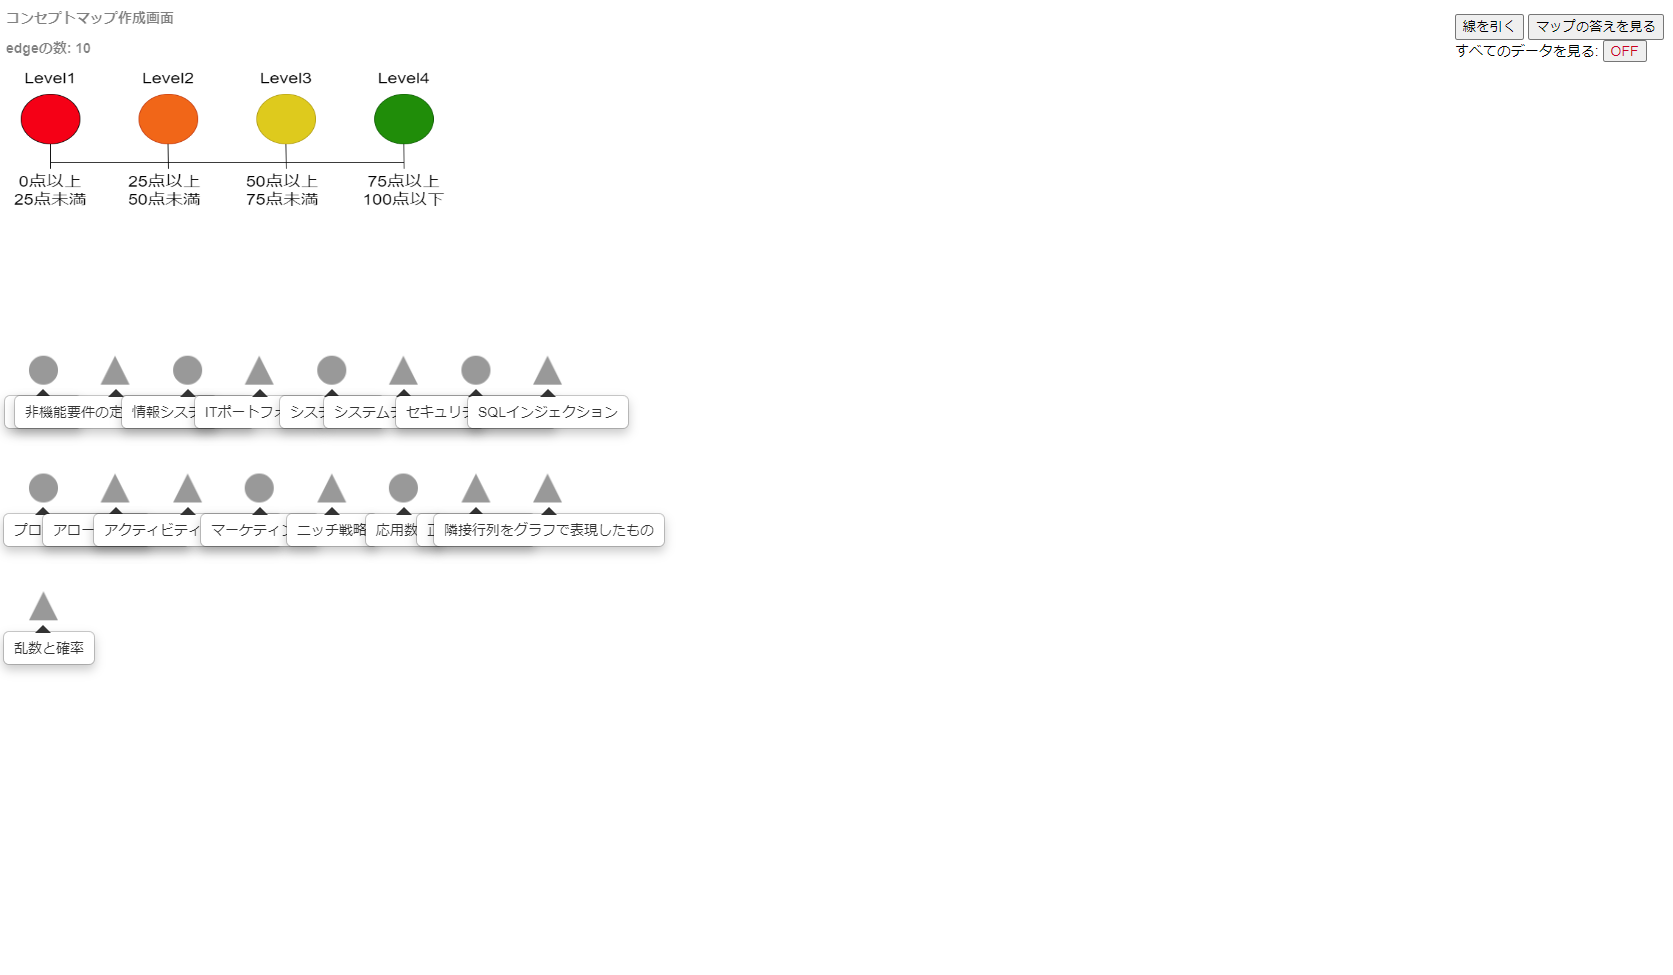
\includegraphics[width=18cm]{img/kasi.eps}
\end{center}
\caption{グラフデータ可視化機能における初期状態のGUI}
\label{fig:kasi}
\end{figure}

学習者は,画面左半分のノードを見ながらコンセプトマップを構築していく.
画面左上部に存在する色の塗られたノードが示すのは獲得点数によるノードの背景色の変化を表している.
これを用いて学習者はノードの背景色を決定する.
また,画面左上部のedgeの数はノードとノード間の結線すべき数を示している.
これにより学習者はノードとノード間に何結線すべきかを確認することができる.

続いて,システムが作成したコンセプトマップを確認した際のGUIを図\ref{fig:kasi_system}に示す.

\begin{figure}[htbp]
\begin{center}
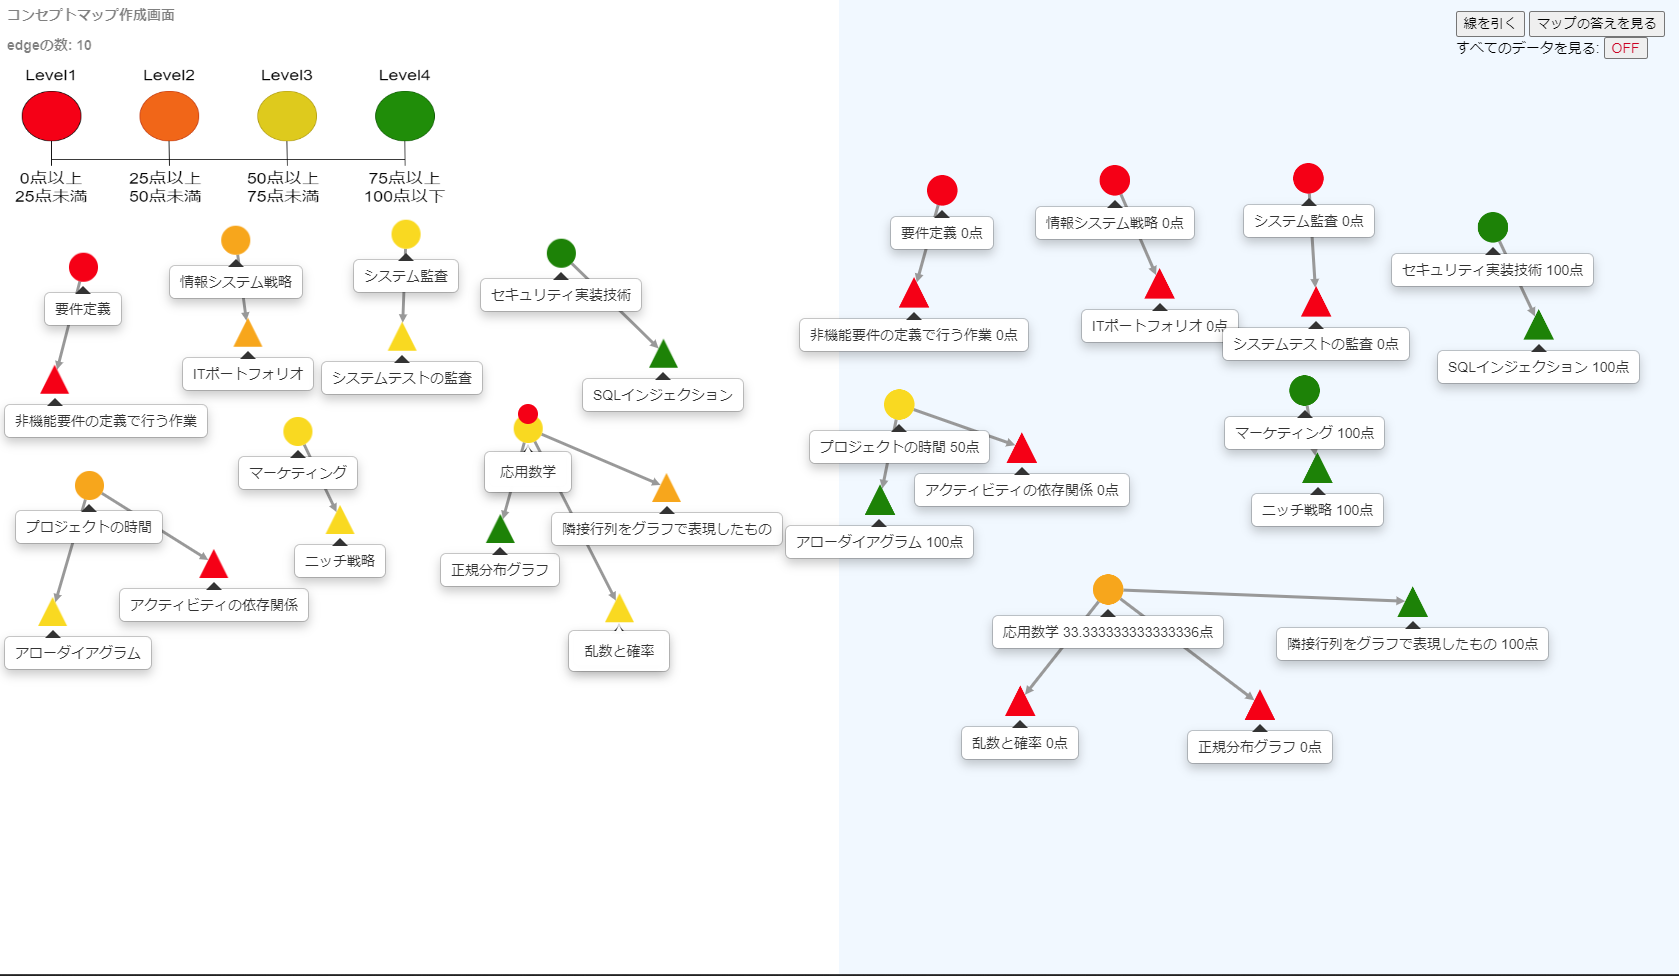
\includegraphics[width=18cm]{img/kasi_system.eps}
\end{center}
\caption{グラフデータ可視化機能におけるコンセプトマップ確認のGUI}
\label{fig:kasi_system}
\end{figure}

システムが自動的に作成したコンセプトマップは画面右側のコンセプトマップである.
これは,画面右上の「マップの答えを見る」ボタンを押下する事により確認できる.
それぞれのノードはあらかじめグラフデータベースに登録されたノードと得点に従ってコンセプトマップと各々のノード背景色が決定されている.
また,ノードの情報として各ノードにおける学習者の得点情報が記載されている.
ただし,親ノードに関する得点は子ノードの平均点の得点となっている.
以上の結果から学習者は自身が作成したコンセプトマップの構造を確認し,コンセプトマップの階層構造自体に誤りがないかどうかの確認と,
自身の主観的知識獲得量と実際の試験の結果から算出された客観的知識獲得量が一致しているかどうかを確認でき,
その結果を基に今後の学習目標設定の基準に本システムを利用できる.
\newpage